\documentclass[11pt]{article}

\usepackage[letterpaper,margin=0.75in]{geometry}
\usepackage{booktabs}
\usepackage{graphicx}
\usepackage{listings}
\usepackage{mathtools}

\setlength{\parindent}{1.4em}

\begin{document}

\lstset{
  language=Python,
  basicstyle=\small,          % print whole listing small
  keywordstyle=\bfseries,
  identifierstyle=,           % nothing happens
  commentstyle=,              % white comments
  stringstyle=\ttfamily,      % typewriter type for strings
  showstringspaces=false,     % no special string spaces
  numbers=left,
  numberstyle=\tiny,
  numbersep=5pt,
  frame=tb,
}

\title{Lab 2 Report}

\author{Dallin Christensen}

\date{February 20, 2014}

\maketitle

\section{Reliable Transport}
I implemented reliable transport by using a sliding window. Packets were sent sequentially from n1 to n2, but were only allowed to be sent if they fell within the scope of the window. Node n1 kept track of how many packets it had sent. As soon as n2 properly received a packet and notified n1 by sending an ACK, n1 would then allow the next packet to be sent (sliding the window up by one packet size).
(all trace statements omitted in these code snippets)
\begin{lstlisting}
def send_if_possible(self):
  if not self.send_buffer:
    return
  if self.unacked_packet_count * 1000 >= self.window_size:
    return
  packet = self.send_one_packet(self.sequence)
  self.increment_sequence(packet.length)
  self.unacked_packet_count += 1
\end{lstlisting}

The sending node (n1 in our case) handled ACKs from the receiving node (n2), making sure to reset the timer every time. It would increase it's ACK number whenever it received a new ACK.
\begin{lstlisting}
def handle_ack(self, packet):
  self.unacked_packet_count -= ((packet.ack_number - self.received_ack_number) / 
                                self.mss)
  self.cancel_timer()
  self.timer = Sim.scheduler.add(
                delay=self.timeout, event='new_ack_data', handler=self.retransmit)
  self.received_ack_number = packet.ack_number
  self.send_if_possible()
\end{lstlisting}

The receiving node (n2) handled packets from the sending node (n1), adding the data it received to a receieve buffer. It would then calculate a cumulative ACK of the highest sequence number it had recieved in order and send that ACK to the sending node.
\begin{lstlisting}
def handle_sequence(self, packet):
  ReliableTransport.stats.add(packet.queueing_delay)
  self.received_sequences.add(packet.sequence)
  self.receive_buffer.append(packet)

  # cumulative ack
  sequence_list = sorted(self.received_sequences)
  for i in range(self.ack/self.mss, len(sequence_list)):
    if sequence_list[i] == self.ack:
      tempPacket = [p for p in self.receive_buffer if p.sequence == self.ack][0]
      self.increment_ack(tempPacket.sequence + tempPacket.length)
      self.app.handle_packet(tempPacket)
  
  self.send_ack()
\end{lstlisting}

The sending node (n1) retransmitted the earliest/lowest (sequentially) packet whenever the timer fired. 
\begin{lstlisting}
def retransmit(self,event):
  if self.received_ack_number < len(self.send_buffer):
    packet = self.send_one_packet(self.received_ack_number)
    self.timer = Sim.scheduler.add(delay=self.timeout, event='retransmit', 
                                    handler=self.retransmit)
\end{lstlisting}

\vspace{0.5cm}
As noted in the tables below, average queueing delay increased and throughput decreased as loss rate increased.
\begin{center}
\begin{tabular}{ c c c c c c c }
  \multicolumn{6}{c}{Testing Results - test.txt} \\
  \hline
  {\tiny Loss Rate} & {\tiny Bandwidth} & {\tiny Propagation Delay} & {\tiny Window Size} & {\tiny Average Queueing Delay} & {\tiny Throughput}\\
  0\% & 10 Mbps & 10 ms & 3000 bytes & 0.000024 sec & 74052.13 bits/sec \\
  10\% & 10 Mbps & 10 ms & 3000 bytes & 0.000024 sec & 38086.53 bits/sec \\
  20\% & 10 Mbps & 10 ms & 3000 bytes & 0.000024 sec & 19509.53 bits/sec \\
  50\% & 10 Mbps & 10 ms & 3000 bytes & 0.00000421 sec & 3780.60 bits/sec \\
\end{tabular}
\end{center}

\begin{center}
\begin{tabular}{ c c c c c c c }
  \multicolumn{6}{c}{Testing Results - internet-architecture.pdf} \\
  \hline
  {\tiny Loss Rate} & {\tiny Bandwidth} & {\tiny Propagation Delay} & {\tiny Window Size} & {\tiny Average Queueing Delay} & {\tiny Throughput}\\
  0\% & 10 Mbps & 10 ms & 10000 bytes & 0.000006990 sec & 2013341.93 bits/sec \\
  10\% & 10 Mbps & 10 ms & 10000 bytes & 0.000006239 sec & 27651.27 bits/sec \\
  20\% & 10 Mbps & 10 ms & 10000 bytes & 0.000004410 sec & 13102.93 bits/sec \\
  50\% & 10 Mbps & 10 ms & 10000 bytes & 0.0000002381 sec & 2645.07 bits/sec \\
\end{tabular}
\end{center}

\vspace{0.5cm}
I did not implement a dynamic retransmission timer.
\vspace{0.5cm}

\section{Experiments}
I experimented with window size by sending the same file (internet-architecture.pdf) over a link with a 10 Mbps bandwidth, 10 ms propagation delay, and 0\% loss rate. I varied the window size and graphed the throughput and average queueing delay for each window size. 

As the window size increases, the average queueing delay of packets increases exponentially.
\begin{center}
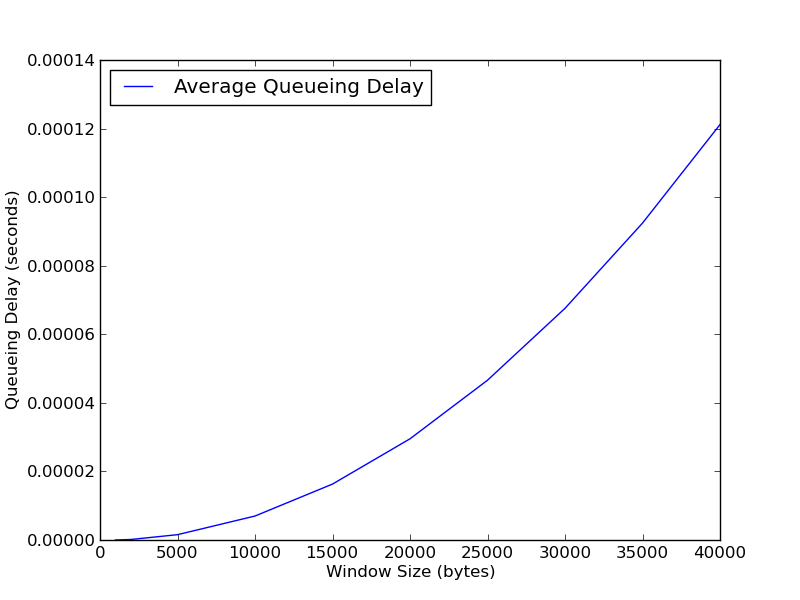
\includegraphics[width=10cm]{../delay.png}
\end{center}

As the window size increases, link throughput increases logarithmically.
\begin{center}
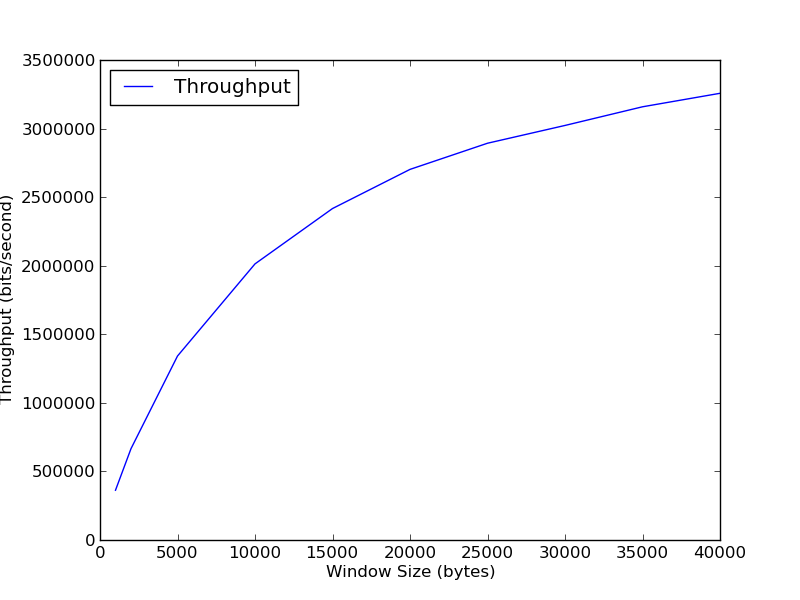
\includegraphics[width=10cm]{../throughputs.png}
\end{center}

\vspace{0.5cm}
\end{document}
